\subsection{Цель выполнения домашнего задания}\label{blockN.VariantM}
\textbf{Цель выполнения домашнего задания }-- \GoalOfResearch

%-------------------------------------------------
\subsection{Задание}
Для цепи Маркова, заданной стохастической матрицей переходов:
\begin{enumerate}
    \item нарисовать граф цепи;
    \item выделить классы существенных и несущественных состояний (вручную – обязательно; программным путём – дополнительное задание для желающих);
    \item рассчитать предельные вероятности для классов существенных состояний;
    \item не выполняя матричных операций с полной стохастической матрицей переходов, записать предельные вероятности в следующих случаях:
    \begin{enumerate}
        \item[4.1] если достоверно известно, что система начинает работу в каком-то одном из состояний (для каждого исходного состояния – свой предельный вектор);
        \item[4.2] если известно, что начальное распределение вероятностей – равновероятное среди всех несущественных состояний;
    \end{enumerate}
    \item провести имитационное моделирование системы, соответствующей рассматриваемой цепи, для этого:
    \begin{itemize}
        \item перебираем все состояния в качестве исходных;
        \item случайно разыграть переход в новое состояние, учитывая распределение вероятностей перехода;
        \item совершить 100 переходов;
        \item подсчитать число вхождений в каждое из состояний системы;
        \item повторить эксперимент 10 раз для каждого исходного состояния;
        \item  построить <<графики>> переключений состояний цепи (для наглядности соединяем дискретные точки);
    \end{itemize}
\end{enumerate}
%-------------------------------------------------
\newpage
\subsection{Решение}
Дана стохастическая матрица переходов $\mathbf{P}$:

$$\mathbf{P}=\begin{pmatrix}
{{ stohast_matr }}
\end{pmatrix}$$

На рисунке \ref{graph} представлен граф переходов, соответствующий матрице $\mathbf{P}$ (состояния из серого кластера в совокупности дают класс несущественных состояний).
\begin{figure}[H]
\centerline{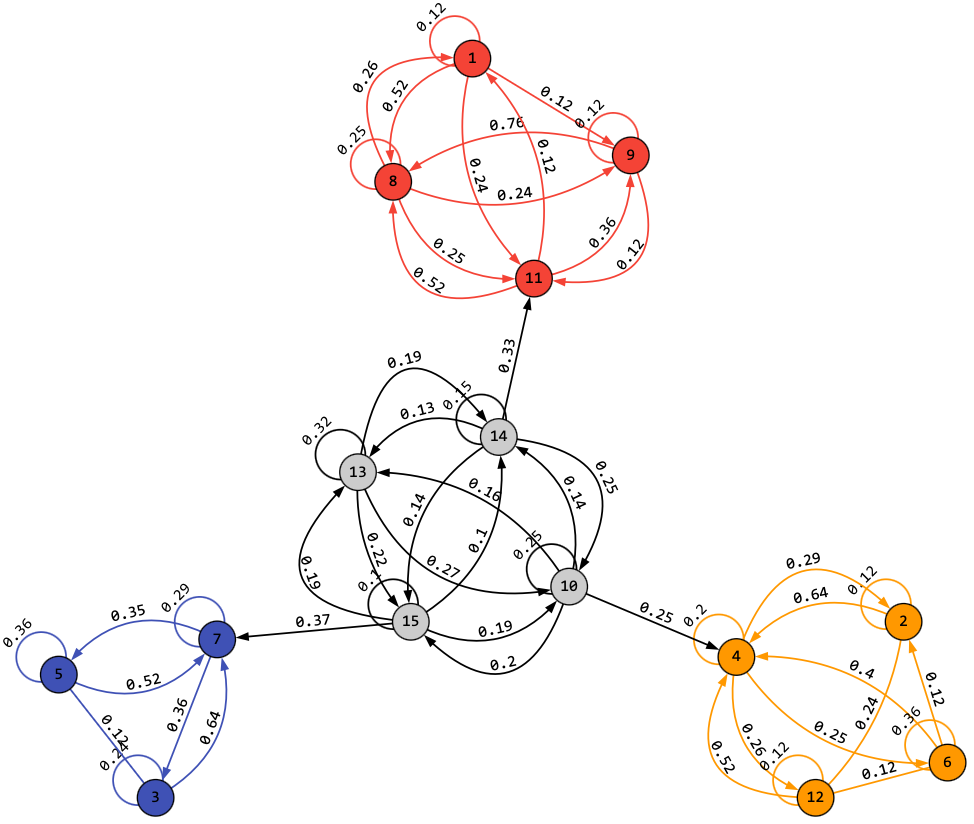
\includegraphics[width=0.7\columnwidth]{Images/1.png}}
\caption{Граф переходов}
\label{graph}
\end{figure}

\subsubsection{Определение вектора предельных вероятностей для классов существенных состояний}

Рассмотрим каждый класс существенных состояний как отдельный марковский процесс.

Была разработана функция, генерирующая матрицу для кластера, заданного списком состояний.

\begin{lstlisting}[language=python, label=prog,caption={\textit{Генерация стахастической матрицы переходов внутри кластера}}]
def make_class_matrix(class_states, P):
    n = len(class_states)
    class_matrix = np.zeros((n, n))
    k = 0

    for i in np.sort(class_states):
        row_prob = []
        for indx in range(len(P[i - 1])):
            if indx+1 in class_states:
                row_prob.append(P[i - 1][indx])
        class_matrix[k] = row_prob
        k += 1

    return class_matrix
\end{lstlisting}

Таким образом имеем 3 матрицы ($\mathbf{P_{1}}, \quad \mathbf{P_{2}}, \quad \mathbf{P_{3}}$) определяющие переходы внутри классов.

$$\mathbf{P_{1}}=
\begin{pmatrix}
    {{ r }}
\end{pmatrix}$$

$$\mathbf{P_{2}}=
\begin{pmatrix}
    {{ g }}
\end{pmatrix}$$

$$\mathbf{P_{3}}=
\begin{pmatrix}
    {{ o }}
\end{pmatrix}$$

~\\

Далее по известной формуле находим вектор предельных вероятностей.

$$(\mathbf{P}^T-\mathbf{E})\times\overline{p}=\overline{0},$$
где $\overline{p}$--вектор предельных вероятностей

Однако, поскольку система является линейно зависимой в качестве последнего уравнения внесем условие $\sum\limits_{i=1}^{n_{vertex}}p_i=1$.

~\\

Была реализована функция, вычисляющая вектор предельных вероятностей  $\overline{p}$.

\begin{lstlisting}[language=python, label=prog,caption={\textit{расчет вектора предельных вероятностей}}]
def marginal_probabilities(P, sum_p=1):
    A = P.T - np.eye(len(P), dtype=float)
    A[-1] = np.full(len(P), 1)
    b = np.zeros(len(P))
    b[-1] = sum_p
    p = np.linalg.solve(A, b)

    return p
\end{lstlisting}

Таким образом, векторы предельных вероятностей:
$$\overline{p}_{1}=( {{ r_vec }} )^T$$
$$\overline{p}_{2}=( {{ g_vec }} )^T$$
$$\overline{p}_{3}=( {{ o_vec }} )^T$$

\subsubsection{Модификация стохастической матрицы}
Для дальнейших вычислений, а также наглядной визуализации результатов моделирования необходимо отсортировать матрицу.

Была реализована функция изменения матрицы по списку состояний.
 \begin{lstlisting}[language=python, label=prog, caption={\textit{Модификация матрицы}}]
def change_matrix(pos, P):
    n = len(P)
    sort_matrix = np.zeros((n, n))
    for i in range(len(P)):
        sort_matrix[i]=P[pos[i]-1]

    sort_matrix = sort_matrix.T
    for i in range(len(sort_matrix)):
        P[i] = sort_matrix[i]
    for i in range(len(P)):
        sort_matrix[i]=P[pos[i]-1]
    return sort_matrix.T
\end{lstlisting}

Граф соответствующий измененной стохастической матрице (для удобства кластеры выделены тем же цветом).

\begin{figure}[H]
\centerline{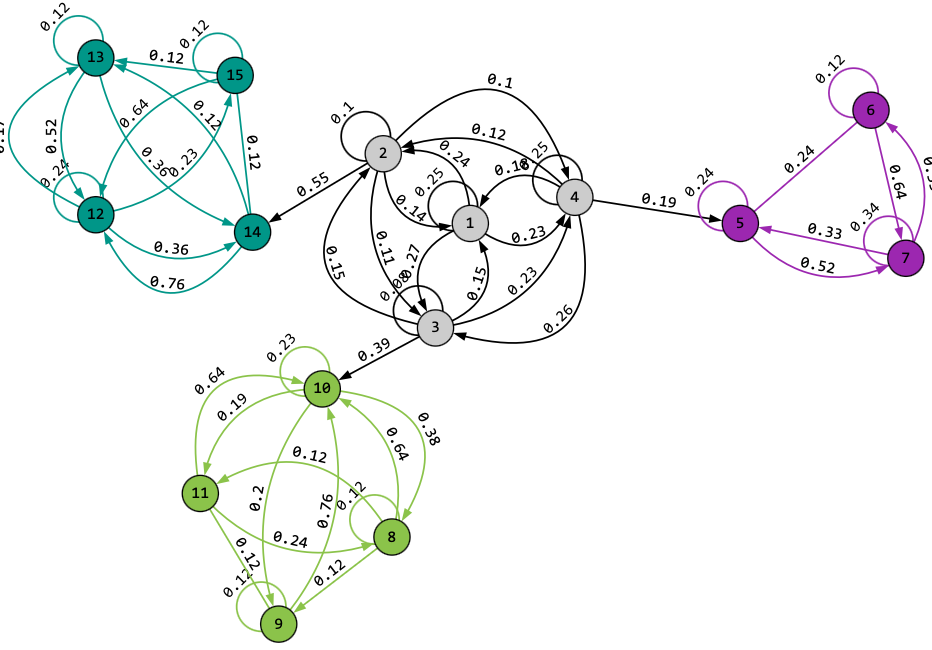
\includegraphics[width=0.8\columnwidth]{Images/2.png}}
\caption{Модифицированный граф}
\label{graph}
\end{figure}


\subsubsection{Определение вектора предельных вероятностей для всех состояний}
Для эффективности вычислений выполним свертку кластеров существенных состояний, представив каждый кластер существенных состояний,
как одно состояние с единичным переходом в самого себя (рисунок \ref{sver_gr}).

\begin{figure}[H]
\centerline{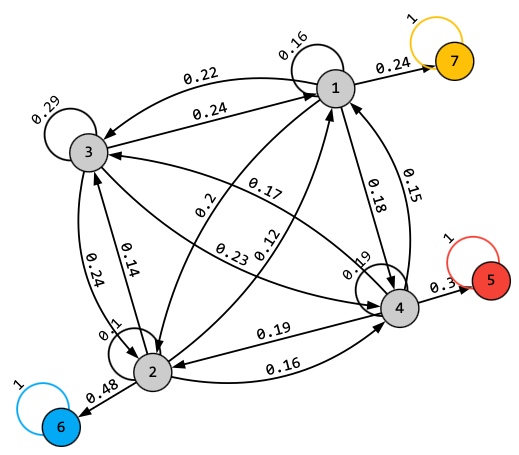
\includegraphics[width=0.7\columnwidth]{Images/3.png}}
\caption{Граф после свертки}
\label{sver_gr}
\end{figure}

Данному графу соответсвует следующая стохастическая матрица переходов:

% Свернутая матрица
$$
\mathbf{P}(n)=
\begin{pmatrix}
{{ P }}
\end{pmatrix}
$$

На основе полученной стохастической матрицы получим предельную матрицу, которая может быть вычеслена следующим образом:

$$
    \mathbf{P} (n) = \mathbf{P}^n
$$

В пределе вероятность оказаться в любом состоянии, пренадлежащем несущественному кластеру, равна 0.
Таким образом можно сформулировать критерий остановки последовательности $\mathbf{P} (n) = \mathbf{P} \cdot \mathbf{P} \cdot \mathbf{P} \cdot \dots$.
Будем считать, что матрица сошлась к предельной, когда сумма вероятностей переходов внутри несущественного кластера будет меньше заданного $\epsilon$.

\begin{lstlisting}[language=python, label=prog,caption={\textit{Нахождение предельной матрицы переходов}}]
    def P_n(P_svert, n):
        eps = 0.0001
        s = 1
        while s > eps:
            P_svert = P_svert.dot(P_svert)
            s = 0
            for j in range(n):
                s += np.sum(P_svert[j][0:n])
        return P_svert
\end{lstlisting}

В результате выполнения функции получена следующая матрица:

$$
\mathbf{P}(n)=
\begin{pmatrix}
 {{ P_n }}
\end{pmatrix}
$$

Далее рассматриваем возможные старты только из состояний, принадлежащих несущественному кластеру
(при старте из любого состояния существенного кластера вектор предельных вероятностей будет состоять из нулей и значений
при рассчете вероятностей для каждого конкретного кластера).

Пусть имеется один кластер несущественных состояний и три кластера существенных состояний, тогда
$$
    \mathbf{P} (n)^T \cdot \pi = (0, \, 0, \, 0 \,...\,x,\, y,\, z)^T,
$$
где $\pi$ - вектор, состоящий из всех нулей за исключением состояния, из которого осуществляется старт (там стоит 1),
$x, y, z$ - предельные вероятности оказаться в одном из существенных кластеров.
Количество лидирующих нулей равно количеству состояний в несущественном кластере.

Таким образом искомые вектора могут быть найдены в виде 
$p = (0,\, 0,\, 0\,...\,x \cdot p_1, y\cdot p_2, z\cdot p_3)^T$.

    \[\overline{p_1} = ({{ ans1_1 }})^T\]

    \[\overline{p_2} = ({{ ans1_2 }})^T\]

    \[\overline{p_3} = ({{ ans1_3 }})^T\]

    \[\overline{p_4} = ({{ ans1_4 }})^T\]

~\\

Найдем вектор предельныех вероятностей если известно, что начальное распределение вероятностей – равновероятное среди
всех несущественных состояний.
Для рассматриваемого случая вектор $\pi$ будет иметь вид $(1/n, 1/n...0, 0,...0)$,
где количество ненулевых элементов равно n - количеству состояний в несущественном кластере, а количество нулевых
позиций соотвествует количеству существенных кластеров.

\[ \overline{p} = ({{ ans2 }})^T\]


\subsubsection{Имитационное моделирование}

Была разработана функция, реализующая переходы, заданное число раз, возвращающая траекторию и список с количеством посещений для каждого состояния (индексы -- состояния).

 \begin{lstlisting}[language=python, label=prog,caption={\textit{реализация марковского процесса}}]
def mark_iter(n, m, states, s_start):
    current_s = s_start
    states_tr = [current_s]
    n_entry = [0 for _ in range(len(states))]
    for _ in range(n - 1):
        per_ver = m[current_s - 1]
        n_entry[current_s - 1] += 1
        next_s = np.random.choice(states, p=per_ver)
        current_s = next_s
        states_tr.append(current_s)
    return n_entry, states_tr
\end{lstlisting}

На рисунке \ref{iter} представлены «графики» переключений состояний цепи.

\begin{figure}[H]
\centerline{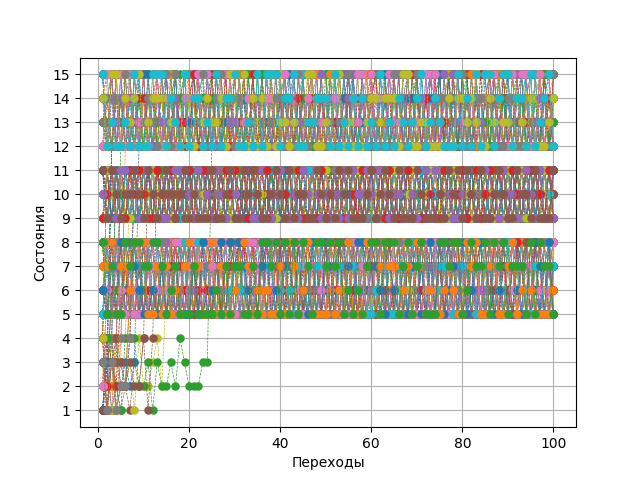
\includegraphics[width=0.7\columnwidth]{Images/iter.png}}
\caption{Переключения состояния цепи}
\label{iter}
\end{figure}

Статистические частоты заключительных состояний моделирования:
$$( {{ lols_tex }} )$$

\begin{lstlisting}[language=python, label=prog,caption={\textit{реализация подсчета частот}}]
def stats(trajectories):
    s = ""
    for tr in trajectories:
        s = s + f"{ round(tr / 150, 3) } ,"
    return s[:-2]
\end{lstlisting}

%-------------------------------------------------
\subsection{Вывод}
В ходе выполнения домашнего задания №2 была проанализирована работа марковского процесса, заданного стохастической матрицей переходов.

% --------------------------------------
% Атрибуты задачи
%\labattributes{}{}{}{}{студент группы \EduGroup, \Author}{\Year, \Semestr}
%--------------

